\chapter{OBC – Computadora de a Bordo}

\section{Diseño de Hardware y Arquitectura Central (OBDH)}
El hardware principal o módulo On-Board Data Handling (OBDH) es el \textit{corazón} de la plataforma INTISAT, concebido de manera específica para coordinar las operaciones vitales, gestión de fallos y comunicaciones.

La arquitectura de procesamiento está basada en un microcontrolador de alto rendimiento \textbf{STM32H7 (144 pines)}, impulsado por osciladores de precisión (Cristal HSE de 24 MHz y LSE de 32.768 kHz). Este núcleo asegura el poder de cómputo necesario para tareas de tiempo real exigidas por las cargas útiles.

\insertfigure{OBC1.jpeg}{0.9}{Diagrama de bloques general de la arquitectura del OBC.}

\subsection{Esquema de Memorias y Almacenamiento}
Para garantizar la persistencia de datos (Housekeeping y rutinas de Payload) y tolerar fallos inducidos por radiación mitigando eventos Single Event Upset (SEU), la OBC implementa un banco de memorias redundante operando a 3.3V:
\begin{itemize}
    \item \textbf{Memorias de Alta Velocidad (x3):} Interconectadas mediante bus QSPI a 133 MHz, priorizando la ejecución rápida y buffers de comunicación.
    \item \textbf{Memorias de Baja Velocidad (x3):} Interconectadas mediante bus SPI tradicional a 25 MHz para redundancia y almacenamiento profundo no volátil.
\end{itemize}

\subsection{Monitoreo Interno y Sensores}
El acondicionamiento físico incluye un banco independiente de \textbf{6 unidades de sensores de temperatura} vinculados directamente al STM32H7 vía bus I2C, lo que permite trazar mapas de calor de la placa madre en tiempo real. 

\section{Capa de Aislamiento e Interfaz de Comunicaciones}
Teniendo en cuenta el entorno disruptivo del espacio, la placa OBC no se comunica directamente con el bus estándar del satélite (PC/104). Se incorpora un diseño de aislamiento galvánico de señales:
\begin{itemize}
    \item Una etapa de \textbf{Banco de Aisladores} protege los puertos expuestos hacia el conector PC/104. Esto involucra puertos críticos de Baja Velocidad (hasta 22 pines GPIO, 2x SPI, 2x I2C y 4x UART utilizados pesadamente por las cargas útiles).
    \item Se incluye un transceptor dedicado para los 2 canales del \textbf{Bus CAN} (CAN H/L), proporcionando inmunidad al ruido y un protocolo robusto para la telemetría cruzada con subsistemas vitales (como el EPS).
\end{itemize}

\section{Máquina de Estados y Modos de Operación}
La OBC gestiona el ciclo de vida de la misión mediante \textbf{cuatro modos de operación} consistentes con el ConOps definido en el Cap.~1: \textit{Inicio}, \textit{Rutina (Nominal)}, \textit{Seguridad (Safe)} y \textit{Decomisión}.

\subsection{Modo Inicio (Deployment y Vuelo Temprano)}
Al eyectarse del inyector P-POD, el \textit{kill-switch} físico libera la energía proveniente del EPS y energiza el satélite. La OBC ingresa al modo de inicio ejecutando la siguiente rutina estricta:
\begin{enumerate}
    \item \textbf{Temporizador de silencio:} ventana obligatoria de \textbf{40~minutos} sin ejecución de hardware crítico ni transmisiones de RF, permitiendo el alejamiento seguro del vehículo lanzador.
    \item \textbf{Checklist de despliegue:} la OBC evalúa los siguientes parámetros:
    \begin{itemize}
        \item Energía: consulta al EPS si la batería supera el 70\,\% de SoC.
        \item Estabilidad orbital: consulta al ADCS para confirmar que las rotaciones residuales están dentro de tolerancia.
    \end{itemize}
    \item Confirmados los niveles, ejecuta el despliegue físico de antenas e ingresa al \textit{Modo Rutina}. Si falla o los niveles no son óptimos, cae por contingencia al \textit{Modo de Seguridad}.
\end{enumerate}

\subsection{Modo Rutina (Operación Nominal)}
Estado operativo estándar. La OBC opera cíclicamente sobre dos frentes simultáneos:
\begin{itemize}
    \item Envía periódicamente (cada órbita por defecto) los datos de telemetría de sanidad (\textit{housekeeping}) de OBC, EPS y radio UHF.
    \item \textbf{Priorización de cargas útiles:} autoriza la ejecución de experimentos científicos (ej. adquisición en microscopía CMOS), almacena los datos transaccionales en el banco de memorias, los empaca vía protocolo interno y los enruta para transmisión hacia tierra.
\end{itemize}

\subsection{Modo de Seguridad (Safe Mode)}
Ante el fracaso del \textit{Modo Inicio} o un evento severo (sub-voltaje, SEU, latch-up), la máquina de estados suspende el Modo Rutina e ingresa al modo de supervivencia:
\begin{enumerate}
    \item \textbf{Corte quirúrgico:} se apagan los puertos a subsistemas y \textit{payloads} no vitales.
    \item \textbf{Transmisión básica:} único envío periódico de telemetría housekeeping (EPS, OBC, UHF).
    \item \textbf{Apuntamiento solar:} ordena al ADCS apuntar los paneles solares al sol de forma sostenida.
    \item \textbf{Interbloqueo:} el satélite queda escuchando telecomandos críticos de tierra (HMAC/SHA) para inyectar correcciones asincrónicas (resets, forzar rutinas, salir del Safe Mode).
\end{enumerate}

\subsection{Modo Decomisión (End of Life)}
Modo de fin de vida, activado mediante telecomando de tierra o por temporizador programado (lifetime expirado). Asegura el cese controlado de operación:
\begin{enumerate}
    \item \textbf{Pasivación de batería:} descarga controlada y desconexión de las celdas para prevenir riesgo de explosión durante reentrada.
    \item \textbf{Apagado de transceptores:} cese definitivo de transmisiones UHF.
    \item \textbf{Latencia mínima:} la OBC entra en \textit{deep sleep}, esperando el reingreso atmosférico natural por arrastre.
\end{enumerate}

\begin{figure}[h]
\centering
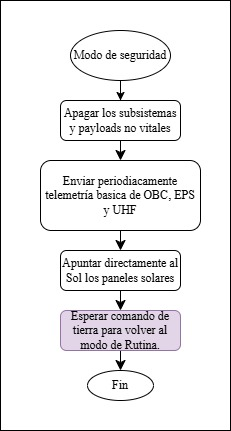
\includegraphics[height=10cm, keepaspectratio]{figures/OBC2.jpeg}
\caption{Flujogramas del modo de operación del satélite.}
\end{figure}
